\chapter{引言}
\label{cha:intro}

\section{大规模集成电路与EDA}

集成电路的产生与发展对人类的社会与工业有着重大而深远的影响。
仅仅在其开发后半个世纪,集成电路变得无处不在,电脑,手机和其他数字电器成为现代社会结构不可缺少的一部分。
这是因为,现代计算,交流,制造和交通系统,包括互联网,全都依赖于集成电路的存在。
甚至很多学者认为有集成电路带来的数字革命是人类历史中最重要的事件。集成电路的成熟将会带来科技的大跃进,
不论是在设计的技术上,或是半导体的工艺突破,两者都是息息相关。

而自从进入大规模集成电路的时代,集成电路一直遵从这摩尔定律的惊人速度而发展着,其中的晶体管数量,
每1.5年增加一倍。近年来,随着制造工艺与材料工艺的持续发展,芯片的规模增速不见放缓。英伟达公司最新
发布的Tesla V100计算卡,在其815平方毫米的面积上,共有210亿颗晶体管,以及5120个CUDA。这张“巨无霸”
计算卡的出现只是集成电路飞速发展的一个缩影。

早期集成电路规模不大,设计复杂度也不高,设计人员甚至可以手工完成集成电路的设计和优化。到了70年代中期,
集成电路的规模不断增加,程序的仿真模拟与逻辑认证开始被引入到集成电路的开发设计中。为此诞生的电子设计自动化
(Electronic Design Automation,EDA)行业也逐步发展。电子设计自动化不仅减少了人工设计带来的差错,而且
大大提高了电路设计的正确性和容错率。然而随着集成电路的发展,EDA领域也迎来了众多挑战:工艺制造技术发展到32纳米
以下所带来的物理效应、增长迅猛的功耗散热问题、信号完整性问题等~\cite{shang2004thermal, swaminathan2010designing}。

\section{集成电路供电网络的分析与设计}

\begin{figure}[H] % use float package if you want it here
  \centering
  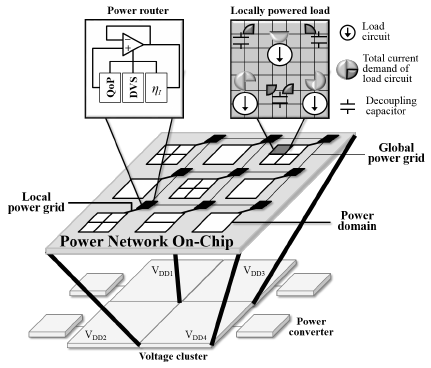
\includegraphics[height=8cm]{power-network-on-chip}
  \caption{集成电路的供电网络}
  \label{fig:figpower}
\end{figure}

在EDA所关注的问题中,集成电路供电网络的设计~\cite{zhu2004power}是比较重要的一个。通过正确的布线,
可以使得外部电源能给芯片上的各个工作单元提供所需的工作电流,以便正常地工作。由于供电网络涉及到电源线网和
地线网这些关键网络,所以它在布线阶段有着比较高的优先级。对于供电网络来说,它经常使用几层乃至十几层的金属进行
供电线网的设计,占用芯片上的相当一部分资源。(要不要提寄生电阻效应和电感效应?)

\begin{figure}[H] % use float package if you want it here
  \centering
  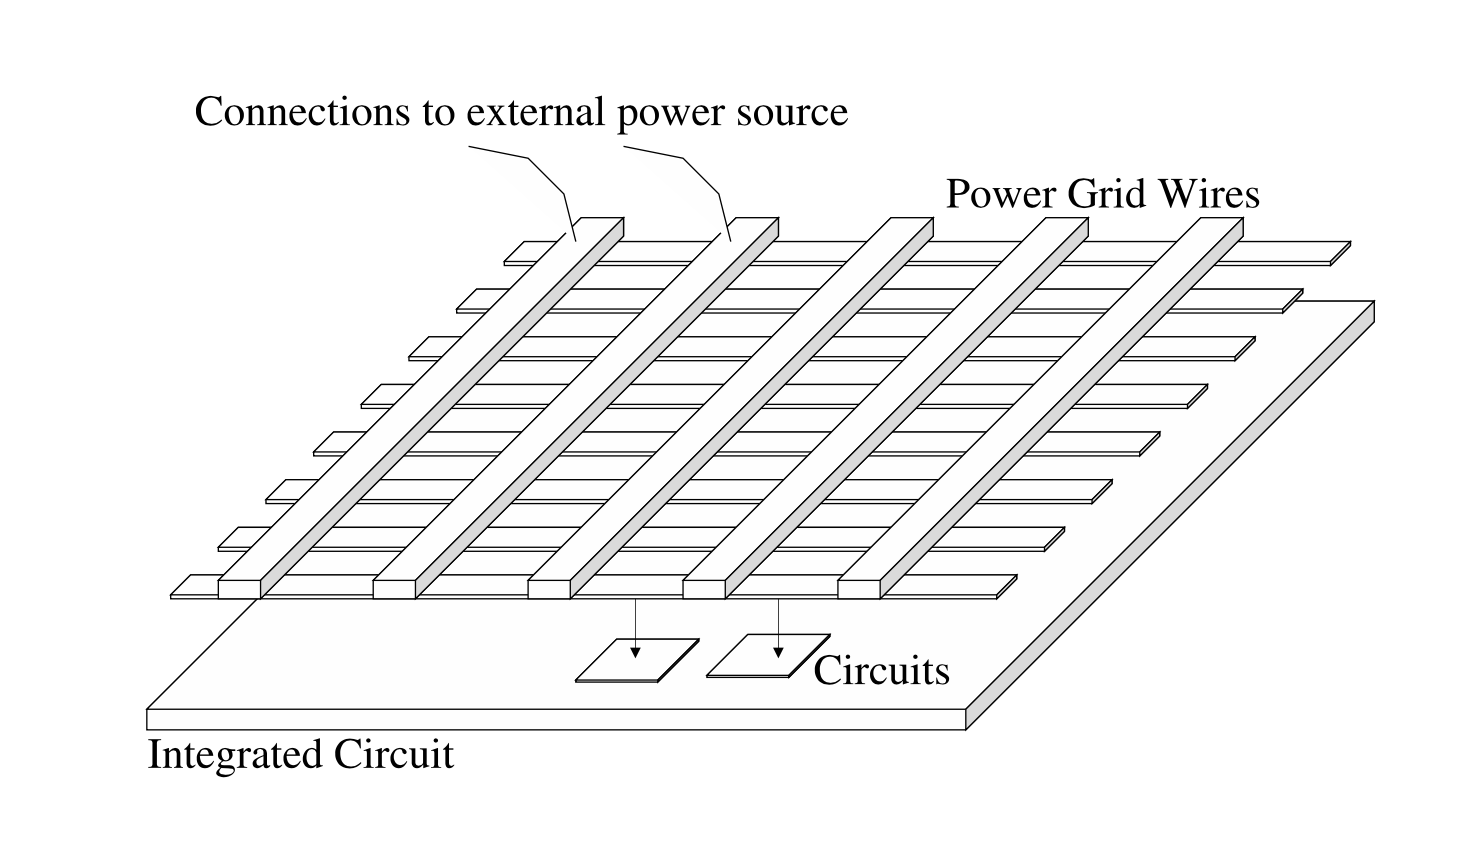
\includegraphics[height=7cm]{power-grid-topology}
  \caption{集成电路的供电网络}
  \label{fig:figtopology}
\end{figure}

目前各种芯片最常用的供电网络基础结构是一个多层的金属的网格状拓扑图~\cite{popovich2007power}。如图\ref{fig:figpower}与图\ref{fig:figtopology}所示。
对供电网络进行静态仿真分析的时候,可以把这个供电网络当做一个纯电阻网络模型,因此可以采用经典的节点分析法~\cite{vlach1983computer}。节点分析方法中,我们通过建立
并求解一个大规模的线性方程组而得到所有电路网络节点的电压值。对供电网络的进行瞬态仿真分析的时候,情况类似。只需要把储能元件的电容和电感进行离散化,使其等效成为一个常数电阻
并联一个电流源即可。而电流源的值由上一个瞬态计算而得。瞬态仿真通过求解每个时间节点上的电路网络方程,可以得出每个时间节点上的每个电路节点的电压响应,从而为仿真提供电路的动态
变化情况。


\section{供电网络设计遇到的挑战}

同样的,随着集成电路的复杂程度日益增长,供电网络的设计也愈加复杂。这主要是因为~\cite{zhu2004power}:
\begin{enumerate}
    \item 芯片制造工艺尺寸不断降低,集成度越来越高,也就是说芯片的功率密度也越来越高,导致了越来越大的开关电流流经供电网络;
    \item 芯片的晶体管数目增多,功率却要控制住,导致供电电压的阈值一定要控制下来;
    \item 由于供电电压的降低,导致晶体管对噪声的容忍度不断下降,也就对供电网络的设计精度提出了更高的要求;
    \item 随着供电网络晶体管密度的上升,金属走线也越来越窄,带来了不能忽视的寄生电阻、寄生电容效应。
\end{enumerate}

如果从一个更实际的角度去考虑这个问题,可以参考下面两种情况:

\begin{itemize}
\item 在设计一个高性能处理核心的时候,分配10%左右的布线资源到供电网络是很常见的一件事情。这么大的布线资源投入是必须的,因为对于处理器来说,经常用1伏特的电压去
产生100瓦特以上的功耗。所以一旦有1毫欧姆的阻抗,那么就会产生100毫伏特的电压降,也就是电压供应的10%;这是不可接受的,会降低6%的处理核心频率,浪费18%的能源分配;
\item 假设处理核心的结构是八层金属网,占据了一个1cm$\times$1cm的面积,并且使用的线宽是$1\mu$。这意味着每一层金属网格有1000条线路。我们进一步假设线网之间的连接
(via)是纯电阻,那么每一层金属网格会有$10^6$个节点。最后整个处理器核心的供电网络就会有大约$8\cdot 10^6$个节点以及$2.4\cdot 10^7$个电阻;可以说是相当复杂的问题;
\end{itemize}

这些因素导致传统的求解方法越来越不能满足现在的设计需求。如果不能很好地上述这些问题,芯片工艺和材料工艺的进步将被供电网络的设计而限制着。此外,随着
设计越来越复杂,设计周期越来越短,所以早期的供电网络规划愈发重要。如果早期供电网络设计是合理的,并有足够的设计余量,那么即使后期设计中出现供电噪声违规的
现象,也可以通过局部小幅度修改而完成设计需求。相反,如果供电网络的早起设计不合理,那么后期再发现问题的时候,就要把前面的所有设计都推倒重来。

本文的研究工作就是基于这样的挑战而展开的额,针对供电网络分析遇到的挑战,主要围绕大规模供电网络的高性能仿真算法开展深入的研究。

\section{供电网络分析基础}

在介绍本论文的算法之前,先对电路分析的数学背景进行基本的介绍。电路系统一般用三大定律进行描述,包括欧姆定律、基尔霍夫电压定律、基尔霍夫电流定律,通过求解其
一阶非线性差分方程来获得电路各节点、支路的响应。但对于规模较大的实际问题,直接列出方程并求解的效率太低。目前主要使用的电路方程构造方案有:

\begin{itemize}
 \item 稀疏表格方法(Sparse Tableau Analysis,STA)~\cite{hachtel1971sparse}由Hachtel等人于1971年提出。此方法构造出来的电路方程包含所有分支电流、
 分支电压以及节点电压的变量。此方法的适用性非常强,系数矩阵非常稀疏,但是要求解的变量较多。
 \item 改进节点分析方法(Modified Nodal Analysis,MNA)~\cite{ho1975modified}由Ho等人于1975年提出。与STA不同的是,MNA所构造的电路方程组只包含电路节点的
 电压变量以及部分支路电流变量,所以所需求解的变量与方程的规模较STA更小。这是目前最常用的方法。
 \end{itemize}

 \begin{figure}[H]
   \centering
   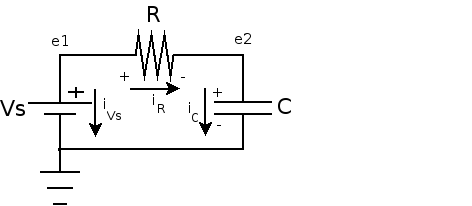
\includegraphics[height=5cm]{simple-circuit}
   \caption{一个简单电路}
   \label{fig:figsimplecircuit}
 \end{figure}

 如图\ref{fig:figsimplecircuit}所示一个简单的电路。如果用电导值$G=\frac{1}{R}$代替电阻值,使用MNA方法可以根据基尔霍夫电压定律列出如下的矩阵方程:

\begin{align*}
 & x=\begin{pmatrix}e_1 & e_2 & i_{V_S}\end{pmatrix}^T, \quad  f=\begin{pmatrix}0 & 0 & V_s \end{pmatrix}^T \\
 \\
 & E=\begin{pmatrix}0&0&0\\ 0&C&0\\ 0&0&0 \end{pmatrix}, \quad A=\begin{pmatrix}G&-G&1\\ -G&G&0\\ 1&0&0 \end{pmatrix}
  \end{align*}

 那么我们可以列出如下的方程:

 \begin{align} E \cdot x'(t) +
  A \cdot x(t) = f \end{align}

 对上列方程进行求解,便可得所求的支路电流值与节点电压值。

 \begin{figure}[H]
   \centering
   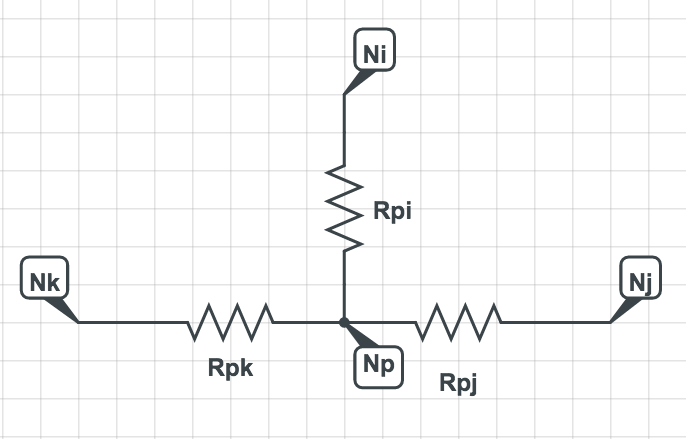
\includegraphics[height=5cm]{mna-demo}
   \caption{改进节点分析方法的系数示意图}
   \label{fig:figmna}
 \end{figure}

 更一般地来说,对于图\ref{fig:figmna}里的一个节点$N_i$来说,它在系数矩阵$A$中对应的元素应该有:

\begin{align}
 \begin{pmatrix}
 & & (i) &  & (j) & & (p) & & (k)& \\
 & & & & & & \vdots & & & \\
 (i) & & & & & & -G_{pi} & & & \\
 & & & & & & \vdots & & & \\
 (j) & & & & & & -G_{pj} & & & \\
 & & & & & & \vdots & & & \\
 (p) & \cdots & -G_{pi} & \cdots & -G_{pj} & \cdots & \sum_{q=\{i,j,k\}} G_{pq}  & \cdots & -G_{pk} & \cdots \\
 & & & & & & \vdots & & & \\
 (k) & & & & & & -G_{pk}& & & \\
 & & & & & & \vdots & & &
 \end{pmatrix}
 \label{Geq}
 \end{align}

也就是说,对于节点$N_p$来说,系数矩阵的第$p$行第$p$列的元素应该是与$N_p$相连的所有电导的和;而其余元素则是对应电导值的相反数。根据这个规则,可以自动化地构造出
电路网络对应的电导矩阵,从而求解电路。

\section{主要工作}

本文的主要工作是根据现有的共轭梯度算法,提出了一种在多机上进行并行计算的加速,并使用多重网格预条件子进行收敛性能的优化。
本文的组成如下:\textbf{第二章}介绍供电网络仿真的相关工作,以及线性方程组求解并行化的研究现状;\textbf{第三章}
介绍了一种基于多重网格预条件子的共轭梯度迭代算法,并提出一种使其在多机上并行计算的方法;
\textbf{第四章}介绍了实验的数据与实验的结果;\textbf{第五章}总结本次毕业设计的工作,回顾不足并展望未来可以继续研究的方向。
